% TODO:
%   - Kijk na of titels in header overflowen
% ----------  
% Questions:
%   - XXX

% https://www.brainlatam.com/blog/wet-dry-active-and-passive-electrodes.-what-are-they-and-what-to-choose-413

% https://www.brainlatam.com/blog/a-brief-introduction-to-eeg-and-the-types-of-electrodes-75

% https://iopscience.iop.org/article/10.1088/1741-2552/abc902/pdf

% bci_review_book_chapter

% In a new chapter, reset the GLS to once again use full version in first occurence
\glsresetall

\chapter{Origins and acquisition of biomedical signals}
\label{ch:biomedical_signals}

% ---------------------------------------------- 
% INTRODUCTION
% ---------------------------------------------- 
\section{Introduction to this chapter}
\label{sec:biomedical_signals_introduction}
% NOTE: "Introduction" exists in each chapter and gives short intro to chapter + what can be expected in chapter

Whilst Chapter \ref{ch:bci} has provided an in-depth intuitive introduction to \glspl{bci}, some more technical aspects need addressing as well to provide a computer scientist with all of the required foundational knowledge for \gls{bci} research.
This chapter provides the required technical knowledge on the data that \gls{bci} systems use, brain signals.
Brain signals are only one of the many types of \gls{biosignal} present in the human body.
Whilst from a computer scientist's perspective brain signals may just be another type of input data to a classification model, having at least a basic understanding of this data is crucial in making good classification algorithms for \gls{bci} systems.
Even when using \gls{dl} approaches where no manual feature engineering has to be done and where basic models without much thought may have pleasing results, understanding the data will allow for the creation of better models.
This understanding of the data also helps in troubleshooting why some models may not have the desired results.

To provide this basic understanding, this chapter starts by briefly discussing \glspl{biosignal} in general.
It is discussed what \glspl{biosignal} are and where they originate from in the human body.
After this general discussion on \glspl{biosignal}, a focus is put on the different \glspl{biosignal} from the human brain, with brain signals measured using \gls{eeg} in particular.
This \gls{eeg} measuring technique and other measuring techniques are also discussed in greater detail.
Whilst it is addressed that \gls{eeg} has some fundamental shortcomings over other measuring modalities, it also has some attractive properties over these alternatives.
These attractive properties are listed and provide an argument as to why the remainder of this master thesis will focus on \gls{eeg} and \gls{mi} \gls{eeg} in particular.

% ---------------------------------------------- 
% ORIGINS
% ---------------------------------------------- 

\section{Biosignals in the human body}
\label{sec:biomedical_signals_biosignals_in_human}

In theory, a \glspl{biosignal} is nothing more than a measurement over time of a living
being.
In practice, these \glspl{biosignal} are closely related to physiological processes.
This makes it possible to monitor or detect those physiological processes using \glspl{biosignal}.
\Glspl{biosignal} can be produced by different energy forms, such as the electrical energy form when measuring \gls{eeg} in \gls{mv}.
Table \ref{tab:biomedical_signals_energy_forms} summarizes some of these energy forms and which type of \glspl{biosignal} they can produce.
Whilst living beings, including humans, produce many different types of \glspl{biosignal}, this master thesis will only consider time-varying electrical \glspl{biosignal}.
These types of \glspl{biosignal}, sometimes reffered to as \gls{elecbiosignal}, are the ones used as input data for \gls{bci} systems.
\Citet{biosignal_definition} discusses these and other types of \glspl{biosignal} in greater detail.

\begingroup
\setlength{\tabcolsep}{6pt} % Default value: 6pt
\renewcommand{\arraystretch}{2} % Default value: 1
\begin{table}[]
    \resizebox{\columnwidth}{!}{%
    \begin{tabular}{|l|p{5cm}|p{7cm}|}
        \hline
        \textbf{Energy form} & \textbf{Variable type}                 & \textbf{Biosignals}                                                                     \\ \hline
        Chemical             & Chemical activity and/or \newline concentration & Blood ions, O2, CO2, pH, hormonal \newline concentrations, and other chemistry                             \\ \hline
        Mechanical           & Position, force, torque or \newline pressure    & Muscle movement or cardiovascular pressures, muscle contractility, valve and other cardiac sounds \\ \hline
        Electrical           & Voltage or current                     & EEG, ECG, EMG, EOG, ERG, EGG, GSR and EDA                                                                 \\ \hline
        Thermal             & Temperature                            & Body temperature and thermography                                                                    \\ \hline
        \end{tabular}%
        }
    \captionsetup{width=0.8\linewidth}
    \captionsetup{justification=centering}
    \caption{Some of the different energy forms in living beings and the measurable biosignals they produce. Data from \citet{biosignal_definition}.}
    \label{tab:biomedical_signals_energy_forms}
\end{table}
\endgroup

% - - - - - - - - - -
% how produced
% - - - - - - - - - -

\subsection{How the human body produces electricity}
\label{subsec:biomedical_signals_biosignals_in_human_how}

Electricity in the human body, better known as bioelectricity, can be seen as the generation or action of tiny electric currents and voltages in physiological processes.
As shown in Table \ref{tab:biomedical_signals_energy_forms}, the measurement of this bioelectricity is what enables the monitoring of \glspl{elecbiosignal}.
This is one of the reasons \glspl{biosignal} are closely related to physiological processes since it measures the bioelectricity used in some of these processes.
A complete understanding of how bioelectricity is made, maintained and transmitted in the human body isn't required for a computer scientist to contribute to the \gls{bci} field.
However, a superficial understanding of this process makes it easier to understand the limits of the accompanied \glspl{elecbiosignal}.
For this reason, the remainder of this section gives a simplified explanation of how bioelectricity is made, maintained and transmitted in the human brain.
This explanation is based on chapter 12 of the recently renewed book by \citet{bioelec_book}, an \gls{eeg} focused explanation of bioelectricity by \citet{eeg_bioelec_creation} and multiple YouTube videos by Neuroscientifically Challenged\footnote{\url{https://youtu.be/tIzF2tWy6KI}}\footnote{\url{https://youtu.be/W2hHt_PXe5o}}\footnote{\url{https://youtu.be/WhowH0kb7n0}}.

% | | | | | | | | | | | | |

\subsubsection{Resting membrane potential causes negatively charged neurons}
\label{subsubsec:biomedical_signals_biosignals_in_human_how_membrane_potential}

As was already addressed in Section \ref{subsec:bci_gaining_popularity_better_measuring}, the human brain has billions of neurons with \citet{neurons_book} stating that around $10^7$ parallel pyramidal neurons reside in only a single $cm^3$ of the brain cortex alone.
A neuron, also known as a nerve cell, is an electrically excitable cell.
Being an electrically excitable cell, a neuron has a resting membrane potential.
This resting membrane potential is around $-70$ \gls{milv} and expresses the difference in electrical charge between the inside and the outside of a neuron.
This negative difference is maintained by the sodium-potassium pump which is responsible for the hydrolysis of ATP to ADP.
During this hydrolysis process the sodium-potassium pump releases three positively charged sodium ions ($Na^+$) whilst only taking in two positively charged potassium ions ($Ka^+$), this difference causes the membrane potential to remain negative.

% | | | | | | | | | | | | |

\subsubsection{Action potential allows for neuron communication}
\label{subsubsec:biomedical_signals_biosignals_in_human_how_action_potential}

Whilst the sodium-potassium pump inside the neuron explains why there is a negative resting membrane potential of around $-70$ \gls{milv}, it doesn't explain the variable volt measurements of \gls{eeg}.
The change in membrane potential occurs when the neuron gets excited.
The most common way a cell gets excited is through the process known as an action potential.
An action potential forms the basis for electrical signalling within neurons, enabling some form of communication between them.
To do this communication, neurotransmitters released by another neuron bind to receptors on the dendrites of the receiving neuron which has a depolarization effect.

This depolarization causes the neuron to become less polarized, resulting in its membrane potential moving close to zero.
When sufficient depolarization occurs, the action potential process could start.
This process is visualised in Figure \ref{fig:biomedical_signals_action_potential}.
For the action potential process to start, the depolarization should be of such a magnitude that the neuron reaches its threshold membrane potential, which is around $-55$ \gls{milv}.
This is achieved through the repeated binding of neurotransmitters to the receptors.
The annotation for "failed initiations" in Figure \ref{fig:biomedical_signals_action_potential} denotes the common situations when the threshold membrane potential is not reached.

When the threshold is reached, a large number of sodium channels open, allowing many positive sodium ions ($Na^+$) into the neuron, causing the membrane potential to rise quickly.
This depolarization is what creates the electrical signal known as the action potential that travels down the neuron to eventually release neurotransmitters itself.
Eventually, a peak is reached, after which the sodium channels close, not allowing any further sodium ions ($Na^+$) to enter the neuron.
To return to its resting membrane potential, the neuron opens its potassium channels to release many potassium ions ($Ka^+$).
This is known as the falling phase where the neuron repolarizes.
However, the release of positive potassium ions ($Ka^+$) happens so quickly that the membrane potential falls below the resting membrane potential.
The neuron is now hyperpolarized, denoted as undershoot in Figure \ref{fig:biomedical_signals_action_potential}.
During this hyperpolarized state, also known as the refractory period, failed initiations occur more often as it is very difficult to fire the neuron again.
Eventually, the resting membrane potential is reached again and the neuron functions like before.


\begin{figure}[ht]
    \centering
    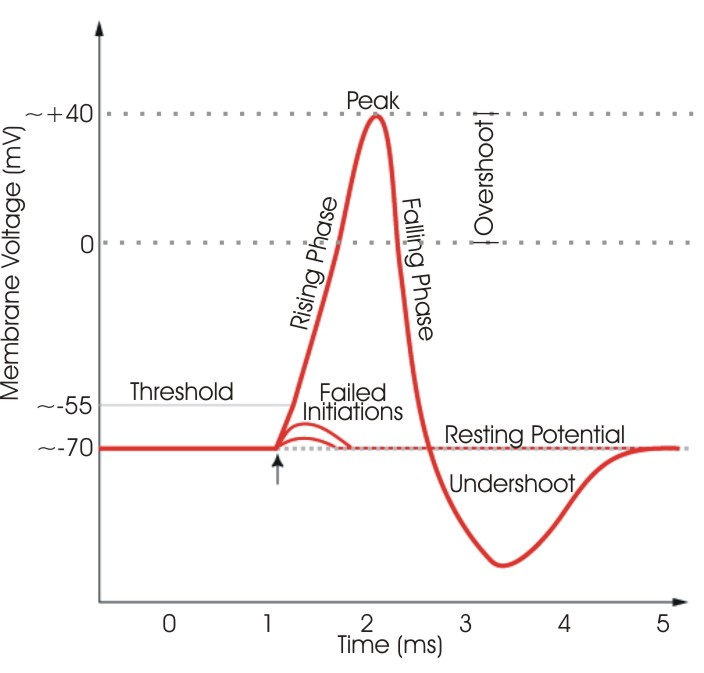
\includegraphics[width=0.7\linewidth]{../images/biosignals/action_potential.jpg}
    \captionsetup{width=0.7\linewidth}
    \captionsetup{justification=centering}
    \caption{Chart of the membrane potential during the action potential process in a neuron. Figure from Synaptidude, GFDL 1.2, via Wikimedia Commons.} 
    \label{fig:biomedical_signals_action_potential}
\end{figure}



% | | | | | | | | | | | | |

\subsubsection{EEG measures postsynaptic potentials}
\label{subsubsec:biomedical_signals_biosignals_in_human_how_postsynaptic_potential}

Whilst the action potential explains how most changes in membrane potential of an individual neuron occur, it is highly unlikely to be measured by \gls{eeg} and other measuring modalities.
This follows from the fact that, as discussed earlier, many billion neurons make up the brain making it impossible to monitor a singular neuron.
Since action potentials are such rapid current flows, it is highly unlikely enough neighbouring neurons will have an action potential at the same time resulting in a measurable signal.
However, whilst it was discussed how neurotransmitters can cause depolarization which can initialize action potentials, these neurotransmitters can also influence the membrane potential in the opposite direction by causing further polarization.
The release of these neurotransmitters and the binding to the receiving neuron also causes currents known as postsynaptic potentials.
Whilst these are not action potentials, they are essentially what causes an action potential to take place and the action potential can also cause the release of neurotransmitters.
These postsynaptic potentials are present for a longer period than action potentials.
Thus, it is more likely for many neighbouring neurons to have active postsynaptic potentials simultaneously.
The summation of these postsynaptic potential currents from many millions of neurons is what is detected by \gls{eeg}.
However, neurons experiencing action potential at that same time are among many other things sources of noise in this summation of these currents.
\Citet{what_eeg_is_and_measures} explain in greater detail what exactly is measured with \gls{eeg}.


% - - - - - - - - - -
% why produced
% - - - - - - - - - -

\subsection{The function of bioelectricity in the human body}
\label{subsec:biomedical_signals_biosignals_in_human_why}

% TODO: start here, short section

% Complete this further but with link to previous on how it is produced

Bioelectricity is omnipresent in the human body. 
The human nervous system relies on bioelectricity to quickly carry \textit{messages} from the human body to the brain and the other way around.
The process of muscle contraction is started when action potentials, which are tiny bursts of bioelectricity, from motor neurons are transmitted to muscle fibres.
\Citet{bioelectricity_baby} explains how bioelectricity even plays a crucial role in developmental biology.
As discussed by \citet{bioelectricity_cancer}, bioelectricity can even be \textit{hijacked} as a way of novel medicine and treatment, i.e. for cancer treatment.
Listing all of the uses for bioelectricity falls outside the scope of this master thesis but it should be apparent that bioelectricity is one of the more vital phenomena in the human body.

% ---------------------------------------------- 
% BIOSIGNALS FROM THE BRAIN
% ---------------------------------------------- 

% TODO 'bci paradigms" 
% info about signals: https://www.e-iji.net/dosyalar/iji_2021_2_48.pdf

\section{Biosignals in the human brain}
\label{sec:biomedical_signals_from_brain}

% \gls{elecbiosignal}
\lipsum[1-2]


% - - - - - - - - - -
% anatomy
% - - - - - - - - - -

\subsection{Anatomy of the brain}
\label{subsec:biomedical_signals_from_brain_anatomy}

% al getoond in bci chapter

\lipsum[1-2]

% - - - - - - - - - -
% Brain waves
% - - - - - - - - - -

\subsection{Brain waves}
\label{subsec:biomedical_signals_from_brain_brain_waves}
% table wolf

\lipsum[1-3]

% - - - - - - - - - -
% Measurable brain activity
% - - - - - - - - - -

\subsection{Common brain signal inducing methods}
\label{subsec:biomedical_signals_from_brain_inducing_methods}

% bci_applications heeft ook overview onder 6. BCI electrical signa

% TODO
% echt uitleggen wat ERP is
% ssvep
% p300 zeker
% MI
% erd

\lipsum[1-7]

% TODO zie chapter 23 bci_handbook
% Issues MI: https://www.frontiersin.org/articles/10.3389/fnins.2021.824759/full
\Gls{mi} is the process in which a person generates brain-activity in the motor cortex merely by imagining motor movements.
\Gls{mi}-based \glspl{bci} are interesting because they don't require any external stimulus nor effective motor movements

\glspl{erp} and the measurable signals they produce, such as the P300 signal, are only one of many sources for detectable brain signals.
In general, \gls{erp} related signals are easier to detect reliably, as the stimulus can be controlled, giving a hint when and where to look for signals and what to look for.

An alternative to \glspl{erp} is using a mental phenomenon called \gls{mi} as source of signals for a \gls{bci} system.
\Gls{mi} is the process in which a person generates brain activity in the motor cortex merely by imagining motor movements.
Section \ref{subsec:biomedical_signals_from_brain_inducing_methods} explains in further detail how \gls{mi} is not dependent on an external stimuli nor actual motor movements.
This makes \gls{mi}-based \glspl{bci} extra appealing as they don't require external stimuli and are applicable for people with motor disabilities.
\Citet{first_mi} were the first to experiment with the idea of using \gls{mi} in an \gls{eeg} classification task.
Since then, many \gls{mi}-based \glspl{bci} have been proposed.
% MI can be trained

% - - - - - - - - - -
% generalisation issues
% - - - - - - - - - -

\subsection{Generalisation issues of brain activity}
\label{subsec:biomedical_signals_from_brain_generalisation}

% neuroplasticity and inter-human variation en non stationarity en mapping brain en... bespreken


\lipsum[1-3]

% ---------------------------------------------- 
% MEASURING BRAIN SIGNALS
% ---------------------------------------------- 

\section{Measuring brain-signals}
\label{sec:biomedical_signals_measuring}

\lipsum[1-2]

% TODO: Different affordable consumer-grade EEG devices have appeared in both Academia (e.g. [5, 6, 7, 8]) and the market (e.g. B-Alert X10, NeuroSky, OpenBCI, Emotiv)
% FROM: cheap_bci_feasibility

% ook zeker herhalen spatial resolution en dat we niet 1 neuron measuren en nooit dat zullen kunnen wss


% There is a wide variety in the devices used for the acquisition of each signal. For EEG, the number of recorded channels (electrodes) varies from a single channel to 64 channels, with sampling frequencies ranging from 128 to 1000 Hz. For the types of electrodes used, there is no dominating type with both wet and dry, and active and passive electrodes being
% hybrid bci bespreken als zijnde combinen sttrenghts: One example of such a hybrid system is to combine EEG and EMG for movement detection (Leeb et al 2011, Loopez-Larraz et al 2018, Tortora et al 2020b), as this allows detection
% uit bci_review_arnau

Many comparisons between different types of measuring equipment, often with greatly differing costs, have already been made \citep{bci_cheap_viability1, bci_cheap_viability2, bci_cheap_viability3, bci_cheap_viability4, bci_cheap_viability5}.
The main consensus is that the cheaper consumer-grade equipment has the potential to reach similar performance of a conventional, often medical-grade, BCI system.
These results are promising but due to the controlled nature of the experiments, they might not reflect real-life applications accurately.
As discussed before, the user experience of a \gls{bci} system is as important if not more important then the raw performance of the system.
% FROM: cheap_bci_feasibility
% OpenBCI1 is an open-source, versatile and affordable biosensing system which can be used to acquire not only EEG signals but also to measure electrical activity of muscle (EMG) and heart (ECG). All OpenBCI boards are based on the open-source electronic platform Arduino with wireless connection to the computer. OpenBCI offers a variety of low-cost amplifiers (boards), electrode systems (e.g. 3D-printed headware) and a software for viewing and recording the biosignals (OpenBCI GUI).2
% as well as from the user’s comfort perspective [4, 13, 14].

% - - - - - - - - - -
% Measuring modalities
% - - - - - - - - - -

\subsection{Measuring modalities}
\label{subsec:biomedical_signals_measuring_modalities}
% EEG ECOG ETC ETC

% Ook inviasive bespreken en wat het is 

% kijk naar wolf ook voor welke types

% bci_applications heeft ook overview onder 5. Signal acquisition

% Several types of EEG paradigms can be distinguished and are discussed in more detail in other reviews of Ramadan and Vasilakos (2017) and Rashid et al (2020).

% ecog: Modalities include the electrocorticogram where electrodes are implanted on the top of the cortex, right under the skull. There is also the possibility to implant electrodes directly in the brain matter (intracortical EEG) to further increase SNR and spatial resolution. However, such invasive approaches fall outside of the scope of this article.

% Alternative signals include magnetoencephalogram (Gross 2019), functional near infrared spectroscopy (Naseer and Hong 2015), and functional Magnetic Resonance Imaging (Sitaram et al 2007). Lesser known signal types are also becoming usable, such as acoustic resonance (Norman et al 2021), which uses the Doppler effect to detect changes in brain activity, and Photoplethysmogram (Han et al 2020), which uses optical reflections to monitor brain activity, in a similar way to near infrared spectroscopy. Another possibility is to monitor spinal cord activity using magnetospinography (Sakakiet al 2020) if one is only interested in lower-limb activity
% UIT bci_review_arnau

% TODO
\lipsum[1-7]

Research by \citet{human_eeg_discovery} is the first in describing the measurement of brain waves from the human skull in a non-invasive manner.
Because of this, the German neuroscientist and psychiatrist Hans Berger is often seen as the inventor of \gls{eeg}.
Whilst he was one of the first to use the term \textit{elektrenkephalogramm}, it was Richard Caton who first described the findings of brain waves in general.
He found this phenomena in animal brains as early as 1875 \citep{first_eeg}.
Since then, \gls{eeg} methodology and equipment has matured and evolved a lot.

% - - - - - - - - - -
% EEG standards
% - - - - - - - - - -

\subsection{Standards for EEG measuring systems}
\label{subsec:biomedical_signals_measuring_standards}

% TODO
\lipsum[1-2]

% - - - - - - - - - -
% available equipment
% - - - - - - - - - -

\subsection{Comparison of available EEG measuring equipment}
\label{subsec:biomedical_signals_measuring_equipment}

% TODO
todo
\lipsum[1-7]

% https://imotions.com/blog/eeg-headset-prices/
% Nextmind 
% Neurosky
% Interaxon
% Muse
% Emotiv
% myBrain
% OpenBCI
% Emotiv EPOC headset

% TODO: citing for sources of img?
% this image was here: https://docs.google.com/document/d/1uaRHNNBJsR8vqT50TllE8s3Jf2dUtAVCcLJb-vhncMM/edit

% - - - - - - - - - -
% artefacts
% - - - - - - - - - -

\subsection{Common EEG artefacts}
\label{subsec:biomedical_signals_measuring_artefacts}

% TODO also discuss how to use them e.g. eye blink as input, ook bespreken niet goed voor e.g. sroke patienten
\lipsum[1-5]

% ---------------------------------------------- 
% CONCLUSIONS OF CHAPTER
% ---------------------------------------------- 
\section{Motivation for using non-invasive MI EEG and chapter conclusions}
\label{sec:biomedical_signals_eeg_motivation_and_summary}
% TODO: summary of this chapter

% uitleggen waarom EEG en MI

\lipsum[1-3]